\documentclass[11pt]{article}
\usepackage[a4paper, margin=2.54cm]{geometry}
\usepackage[utf8]{inputenc}
\usepackage[spanish, mexico]{babel}
\usepackage[spanish]{layout}
\usepackage[article]{ragged2e}
\usepackage{textcomp}
\usepackage{amsmath}
\usepackage{amssymb}
\usepackage{amsfonts}
\usepackage{proof}
\usepackage{bussproofs}
\usepackage{graphicx}
\usepackage{enumerate}
\usepackage{multirow}

\setlength{\parindent}{5pt}

\title{
    Entrega 2 \\
    \large Sistemas Operativos II}
\author{Mellino, Natalia \and Farizano, Juan Ignacio}
\date{}

\begin{document}
\maketitle
\noindent\rule{\textwidth}{1pt}

\begin{enumerate}[1)]
  \section*{Historia}
%==============================================================================
% Ejercicio 1
%==============================================================================
  \item[\textbf{1)}]  
    \begin{itemize}
      \item \textbf{Multitarea, pero monocontexto:}
        Con la introducción de sistemas con capacidades multitareas los usuarios
        se han acostumbrado a que sus equipos hagan muchas cosas al mismo tiempo.
        En los dispositivos móviles nos encontramos con una fuerte reducción en
        las expectativas de multitarea. Esto es debido a dos motivos: la primera,
        es que como los dispositivos móviles carecen de memoria virtual, la memoria 
        disponible se convierte en un recurso escaso y el SO se ve obligado a limitar el
        número de procesos en ejecución. La segunda razón radica en el modelo de uso
        de los dispositivos móviles: comparadas a las pantallas de equipos de escritorio
        éstas son mucho más pequeñas, por lo tanto las interfaces abandonan el modelo 
        de interacción WIMP así como la \emph{metáfora del escritorio} para volver a la de un
        sólo programa visible en todo momento.
        
      \item \textbf{El jardín amurallado:} como consecuencia indirecta del lanzamiento
      de las plataformas móviles se tiene la popularización de un modelo de distribución
      de software conocimo como \emph{plataforma cerrada} o jardín amurallado. Inicialmente fue 
      Apple quién lanzó su tienda de aplicaciones conocida como \emph{App Store}. La 
      peculiaridad de esto radica en que si bien cualquier desarrollador puede crear una
      aplicación y enviarla, Apple se reserva el derecho de aprobarla o eliminarla en
      cualquier momento.

      Inmediatamente siguieron los mismos pasos Android con \emph{Google Play} y Microsoft 
      con \emph{Windows Phone Store}. 

      Este modelo de autorización y distribución de software rompe con lo que Jonathan Zittrain
      define como la \emph{generatividad} de los equipos de cómputo y de la red en general.
    \end{itemize}
%==============================================================================
    \begin{enumerate}[(a)]
      \item \textbf{Falso.} La mayor parte de los sistemas operativos históricamente
            han sido \emph{monolíticos.}
      \item \textbf{Verdadero.} Un sistema con organización híbrida es mayormente
            monolítico pero maneja algunos procesos que parecerían centrales mediante
            procesos de nivel usuario como los microkernel.
      \item \textbf{Falso.} En los sistemas monolíticos hay un sólo proceso
            privilegiado que opera en modo supervisor, y dentro del cual se encuentran
            todas las rutinas para las diversas tareas que realiza el sistema operativo.
      \item \textbf{Falso.} El núcleo del sistema operativo se mantiene en el mínimo
            posible de funcionalidad.
      \item \textbf{Falso.} A medida que los sistemas operativos y los programas
            crecieron en tamaño, fue necesario abstraer el espacio de almacenamiento
            para dar la ilusión de que se cuenta con más memoria de la que realmente
            se tiene. Así surge el concepto de memoria virtual. Por lo tanto, no está
            relacionado directamente con el surgimiento de las computadoras personales,
            sino con el crecimiento del tamaño de los programas y sistemas operativos. 
      \item \textbf{Verdadero.} En los sistemas multiprogramados, diferentes tipos
            de procesos pueden tener distinto nivel de importancia, esto requiere
            la implementación de diversas prioridades para cada uno de éstos.
    \end{enumerate}
%==============================================================================
% Ejercicio 2
%==============================================================================
  \item[\textbf{2)}] Indicamos cuáles arquitecturas y cuáles sistemas operativos 
  se utilizan mayoritariamente para ciertos usos en el siguiente cuadro: 
  \begin{figure}[h!]
    \begin{center}
      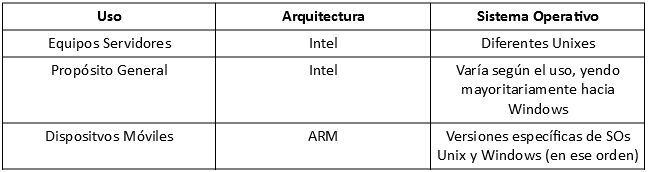
\includegraphics[width=0.85\linewidth]{unknown.png}
    \end{center}
  \end{figure}
      % \begin{tabular}{| c | c | c |}
      % \hline
      % \textbf{Uso} & \textbf{Arquitectura} & \textbf{SO} \\ \hline
      % \textbf{Equipos servidores} & Intel & Diferentes Unixes \\ \hline
      % \textbf{Propósito general} & Intel & Varía según el uso, yendo mayoritariamente hacia Windows\\ \hline
      % \textbf{Dispositivos móviles} & ARM & Versiones específicas de SOs Unix y Windows (en ese orden).\\ \hline
      % \end{tabular}
%==============================================================================
% Ejercicio 3
%==============================================================================
    \section*{Procesos}
    \item[\textbf{3)}]   
      \begin{enumerate}[(a)]
        \item \textbf{Verdadero.} Basta con ejecutar un programa más de una vez,
              por cada vez que se ejecuta se crea un proceso nuevo relacionado
              al mismo programa.
        \item \textbf{Falso.} Cada proceso está asociado a un sólo programa, ya que
              por definición de proceso éste es la imagen en memoria de un programa
              en ejecución.
        \item \textbf{Falso.} Un programa es un conjunto de instrucciones, es decir,
              el código fuente en sí. En cambio, una tarea o proceso es el programa
              cargado en memoria y en ejecución.
      \end{enumerate}
%==============================================================================
% Ejercicio 4 
%==============================================================================
    \item[\textbf{4)}]
    Como ahora en los sistemas operativos se usan las multitareas apropiativas, la velocidad
    de cambio entre una tarea y otra es mucho más rapida ya que con el objetivo de dar la
    ilusión de uso exclusivo de la computadora, el hardware emite periódicamente al sistema
    operativo interrupciones (señales) que le indican que cambie el proceso activo.
    De esta forma, al usuario le parece que las tareas se están ejecutando simultáneamente
    cuando en verdad solo es ejecutada una al mismo tiempo durante un periodo
    de tiempo muy corto antes de pasar a la siguiente.
\end{enumerate}

\end{document}